\usetikzlibrary{arrows}

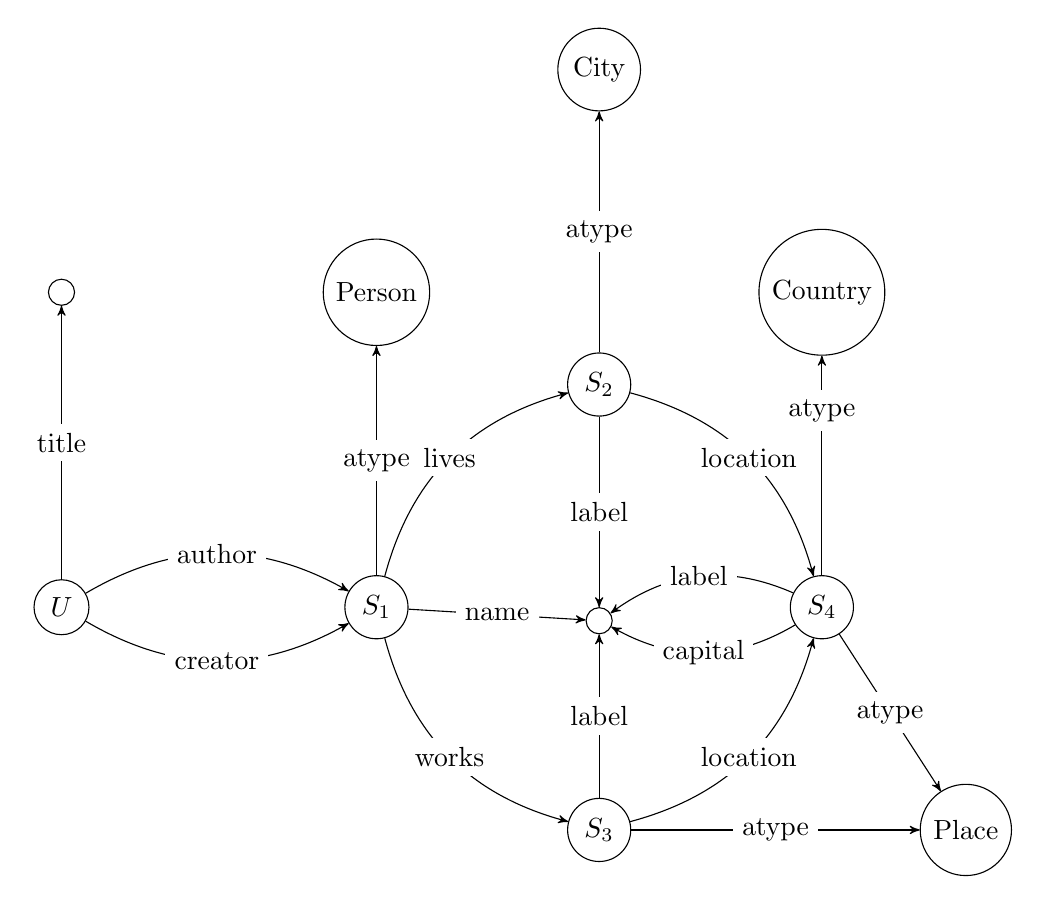
\begin{tikzpicture}[->,>=stealth',node distance=4cm]
\node [draw,circle] (b) {$\mathfrak{U}$};
\node [draw,circle,right of = b] (h1) {$S_1$};
\node [draw,circle,above right of = h1] (h2) {$S_2$};
\node [draw,circle,below right of = h1] (h3) {$S_3$};
\node [draw,circle,above right of = h3] (h4) {$S_4$};
\node [draw,circle,above of = h1] (person) {Person};
\node [draw,circle,above of = h2] (city) {City};
\node [draw,circle,above of = h4] (country) {Country};
\node [draw,circle,below right of = h4,xshift=-1cm] (place) {Place};
\node [draw,circle,above of = b] (c1) {$\varnothing$};
\node [draw,circle,below of = h2,yshift=1cm] (c2) {$\varnothing$};

\path
(b) edge node[fill=white] {title} (c1)
(h1) edge node[fill=white] {name} (c2)
(h3) edge node[fill=white] {label} (c2)
(h2) edge node[fill=white] {label} (c2)
(h4) edge[bend right] node[fill=white] {label} (c2)
(h4) edge[bend left] node[fill=white] {capital} (c2)

(h1) edge node[fill=white] {\glssymbol{atype}} (person)
(h2) edge node[fill=white] {\glssymbol{atype}} (city)
(h4) edge node[near end,fill=white] {\glssymbol{atype}} (country)
(h4) edge node[fill=white] {\glssymbol{atype}} (place)
(h3) edge node[fill=white] {\glssymbol{atype}} (place)
(h1) edge[bend left] node[fill=white] {lives} (h2)
(h1) edge[bend right] node[fill=white] {works} (h3)
(h2) edge[bend left] node[fill=white] {location} (h4)
(h3) edge[bend right] node[fill=white] {location} (h4)
(b) edge[bend right] node[fill=white] {creator} (h1)
(b) edge[bend left] node[fill=white] {author} (h1)
;
\end{tikzpicture}